A radar station can be used to deduce the speed of an airplane. The radar station measures the distance $s$ to the airplane in km. The airplane is cruising at a height of 6km above the ground. The radar station finds that $s$ is decreasing at a rate of $400$km per hour when $s=10$km.
\begin{figure}[H]
	\centering
	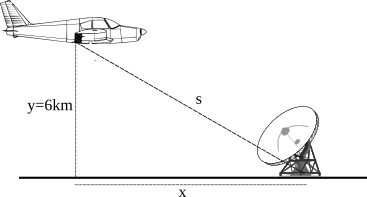
\includegraphics{plane_radar1}
\end{figure}
\begin{enumerate}
	\item When $s=10$km, write down $\frac{ds}{dt}$
	\item The altitude of the plane is not changing. Write down $\frac{dy}{dt}$.
	\item Use Pythagoras' Theorem to write down the relationship between the values of $x$, $y$ and $s$
	\item Hence find $x$ when $s=10$
	\item The displacement of the airplane from the tower is denoted $x$, write down how we would denote the speed of the airplane.
	\item Hence, using rates of change, find the horizontal speed of the airplane in km per hour.
\end{enumerate}
